\documentclass[12pt]{article}

\usepackage{graphicx}
\usepackage[margin=0.75in]{geometry}
\usepackage{multirow}

\begin{document}

\section*{#3 (a)}

\noindent The density function for the Weibull is 
\[ f(x|\alpha, \lambda) = \alpha\lambda x^{\alpha-1} \exp(-\lambda x^\alpha) \]
with survival function
\[ S(x|\alpha, \albmda) = \exp(-\lambda x^\alpha). \]
\noindent We retain 20,000 posterior samples after a burn-in of 5000. There didn't seem to be any issues regarding convergence.
\bigskip

\noindent I use four different sets of priors:
\begin{enumerate}
\item $p(\alpha)\propto 1/\alpha$, $p(\lambda)\propto 1/\lambda$
\item $\alpha\sim Ga(1, 1)$, $\lambda\sim Ga(1, 1)$
\item $\alpha\sim Ga(1, 1/10)$, $\lambda\sim Ga(1, 1/10)$
\item $\alpha\sim Ga(50, 50)$, $\lambda\sim Ga(50, 50)$
\end{enumerate}
\noindent My preferred set is number 1, since this is non-informative while still not producing an improper posterior. Set 3 is also fairly non-informative, but is a proper prior. Sets 2 and 4 both give priors means to 1 for both parameters, but differ greatly in the prior variance (2 has much larger variance relative to 4).
\bigskip

\noindent From the figures, only prior set 4 gives much different results than the other 3, which is expected since set 4 is intended to be highly informative.
\bigskip

\noindent The posterior for $\alpha$ is each ploidy group is very similar across all prior sets (note the degree of overlap in the distributions). It may be reasonable to conclude that the value for $\alpha$ is common across the two groups.
\bigskip

\noindent The following table provides a numerical summary for the posteriors in each ploidy group under prior set 1.
\bigskip

\begin{table}[h]
\centering
\begin{tabular}{ll|rrrr} \hline\hline
Profile & Param & \multicolumn{1}{l}{mean} & \multicolumn{1}{l}{var} &
    \multicolumn{2}{l}{hpd} \\ \hline
\multirow{2}{*}{Aneuploid} & $\alpha$  & 0.827 & 0.015 & 0.584 & 1.066 \\
                           & $\lambda$ & 0.114 & 0.001 & 0.047  & 0.191 \\ \hline
\multirow{2}{*}{Diploid}   & $\alpha$  & 0.774 & 0.018 & 0.513 & 1.050 \\
                           & $\lambda$ & 0.221 & 0.006 & 0.083  & 0.385 \\ \hline\hline
\end{tabular}
\caption{Posterior summaries under prior set 1.}
\end{table}

\begin{center}
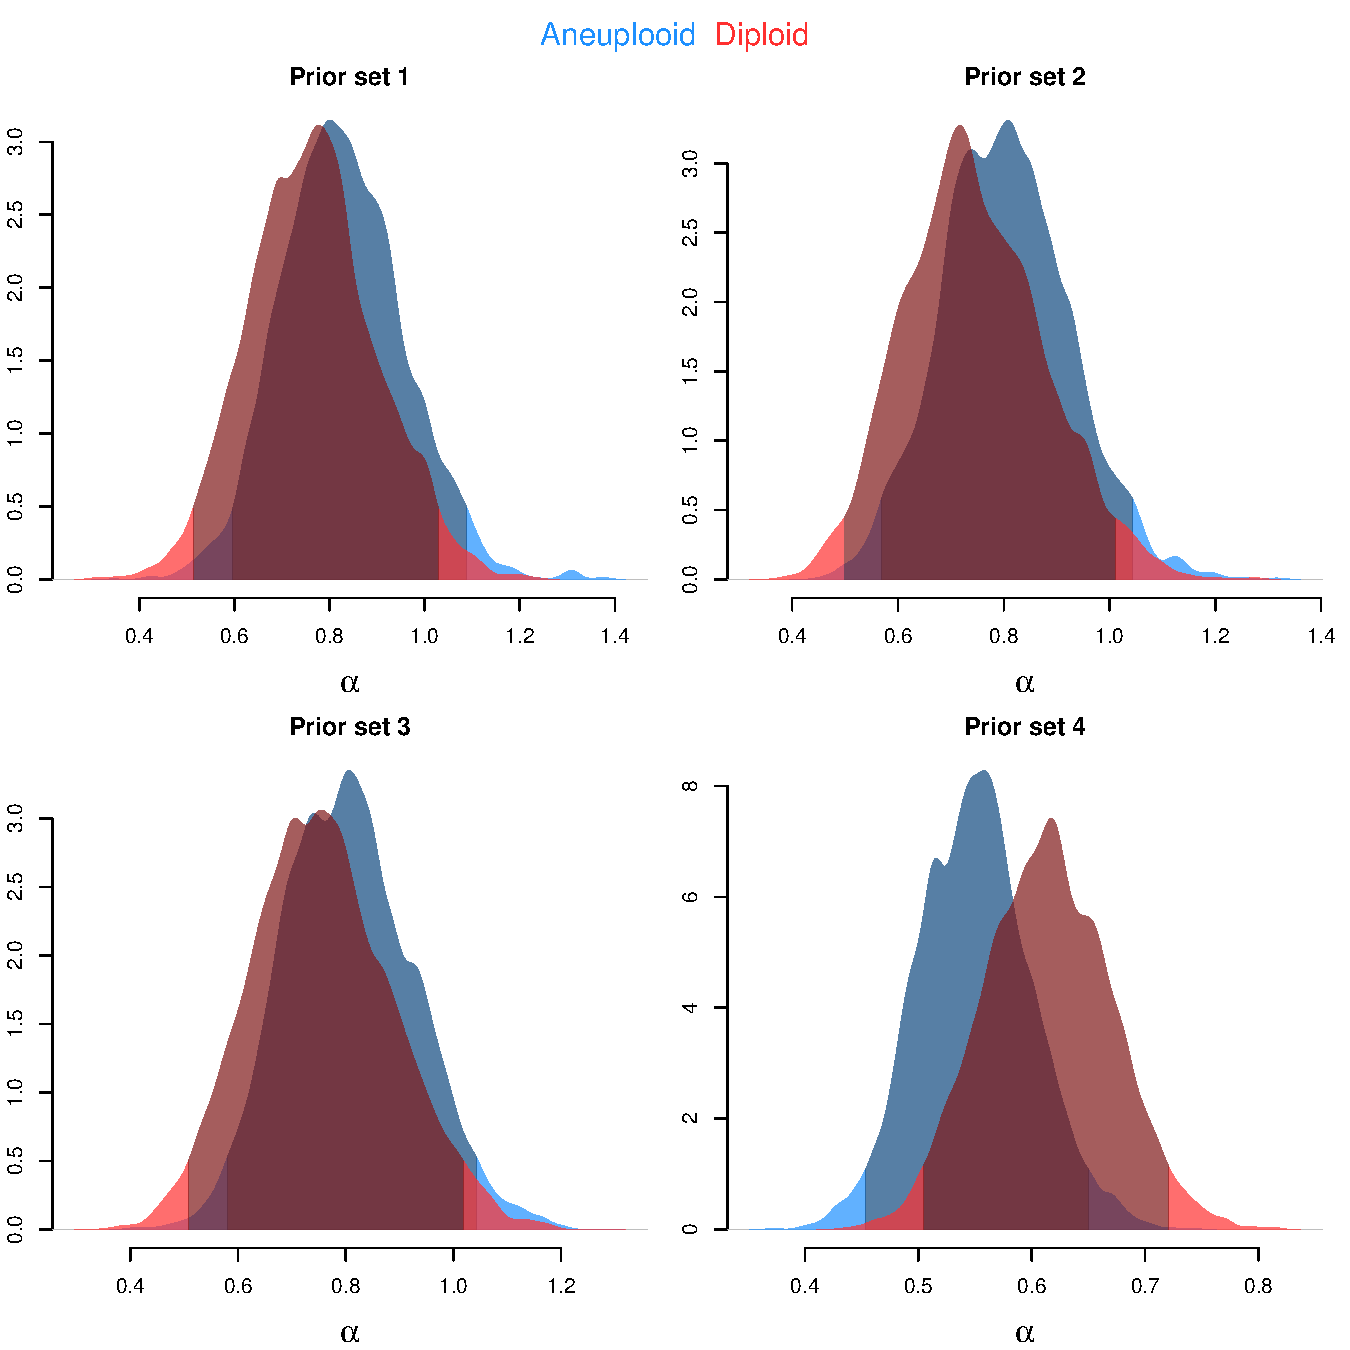
\includegraphics[scale=0.50]{a_sens_alpha.pdf}
\bigskip
\bigskip

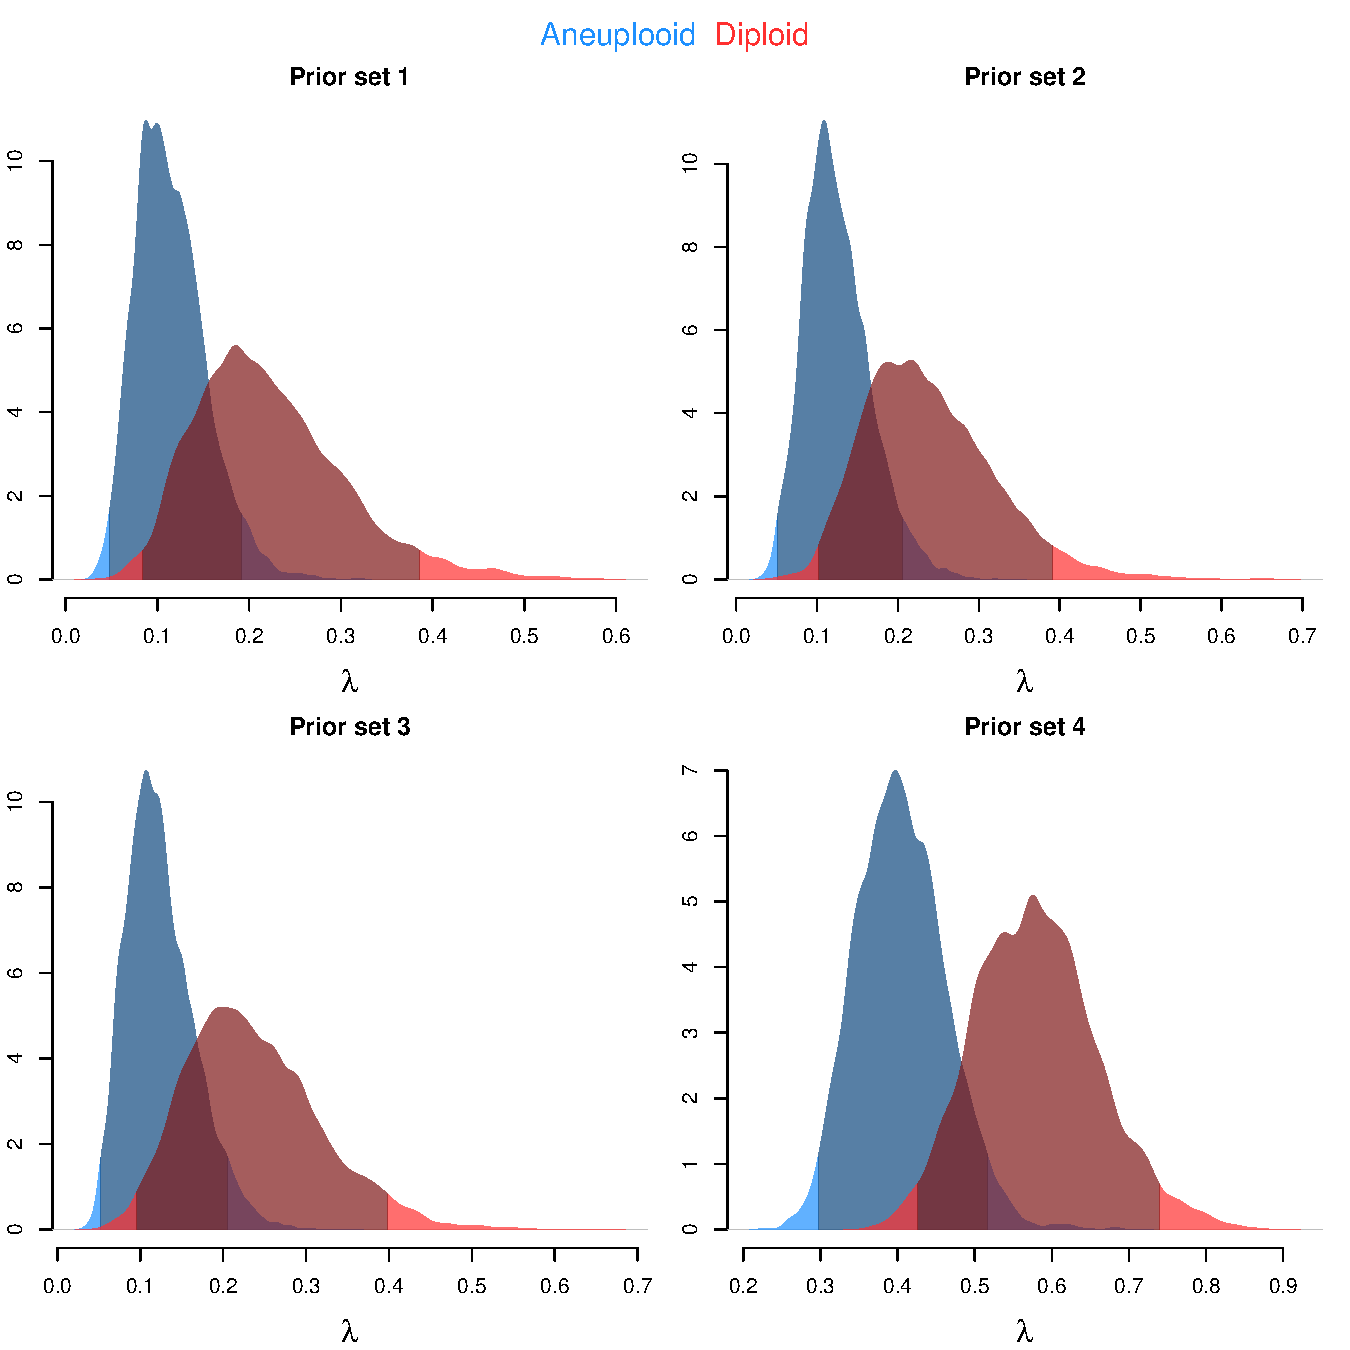
\includegraphics[scale=0.50]{a_sens_lambda.pdf}
\end{center}

\section{3 (b)}

\end{document}
